
% Setting up the document class for Beamer
\documentclass{beamer}

% Including essential packages
\usepackage[utf8]{inputenc}
\usepackage[T1]{fontenc}
\usepackage{lmodern}
\usepackage{tikz} % For drawing the box with text
\usepackage{array} % For table formatting

%%%%%%%%%%%%%%%%%%%%%%%%%%%%%%%%%%%%%%%%%%%%%%%%%%%%%%%%%%%%
%% Paquetes.. %%%%%%%%%%%%%%%%%%%%%%%%%%%%%%%%%%%%%%%%%%%%%
\usepackage[latin1]{inputenc}
%\usepackage{pstricks,pstricks-add,pst-node,pst-text,pst-3d}
\usepackage{amsmath}
\usepackage{cancel}
%% Mate
\usepackage{pst-func}
\usepackage{pst-math}


% Configuring the Beamer theme
\usetheme{Madrid}
\usecolortheme{beaver}

% Defining the title and author
%% Libreria de formulas %%%%%%%%%%%%%%%%%%%%%%%%%%%%%%%%%%%%
%% Velocidad en el Mov. Rec. Uniforme %%%%%%%%%%%%%%
\def\vmru{
%% Eq. 1 %%%%%%%%%%%%%
\begin{equation}
v=\frac{x}{t}
\label{vmru}
\end{equation}
%%%%%%%%%%%%%%%%%%%%%%%%%%%%%%%%%%%%%%%%%%%%%%%%%%%%
}

%% Distancia en el Mov. Rec. Uniforme %%%%%%%%%%%%%%
\def\xmru{
%% Eq. 2 %%%%%%%%%%%%%
\begin{equation}
x=vt
\label{xmru}
\end{equation}
%%%%%%%%%%%%%%%%%%%%%%%%%%%%%%%%%%%%%%%%%%%%%%%%%%%%
}

%% Tiempo en el Mov. Rec. Uniforme %%%%%%%%%%%%%%%%%
\def\tmru{
%% Eq. 3 %%%%%%%%%%%%%
\begin{equation}
t=\frac{x}{v}
\label{tmru}
\end{equation}
%%%%%%%%%%%%%%%%%%%%%%%%%%%%%%%%%%%%%%%%%%%%%%%%%%%%
}

%% Libreria de Notas    %%%%%%%%%%%%%%%%%%%%%%%%%%%%%%%%%%%%
%%%%%%%%%%%%%%%%%%%%%%%%%%%%%%%%%%%%%%%%%%%%%%%%%%%%
%%%%%%%%%%% NU para la velocidad %%%%%%%%%%%%%%%%%%%
%%%%%%%%%%%%%%%%%%%%%%%%%%%%%%%%%%%%%%%%%%%%%%%%%%%%
\def\vNUa%
{
%% Dibuja una cajita!! %%%%%%%%%%%%%%%%%%%
%% el background de gris..
\psframebox[linewidth=2pt,framearc=.3,fillstyle=solid,
fillcolor=lightgray]{
\begin{tabular}{c}
%%%%%%%%%%%%%%%%%%%%%%%%%%%%%%%%%%%%%%%%%%
{\bf Notas de Unidades}\\
{\sc magnitud}: Velocidad [v].
La velocidad puede venir en: \\

$\frac{{\rm km}}{{\rm h}}$ ; 
$\frac{{\rm m}}{{\rm s}}$ ; 
$\frac{{\rm cm}}{{\rm s}}$. \\

$1~\frac{{\rm km}}{{\rm h}}=
\frac{1000}{3600}~\frac{{\rm m}}{{\rm s}}
=\cancelto{0.277}{\frac{1}{3.6}}\frac{{\rm m}}{{\rm s}}$ \\

$1~\frac{{\rm m}}{{\rm s}} = 100~\frac{{\rm cm}}{{\rm s}}$

%%%%%%%%%%%%%%%%%%%%%%%%%%%%%%%%%%%%%%%%%%
\end{tabular}
}
%%%%%%%%%%%%%%%%%%%%%%%%%%%%%%%%%%%%%%%%%%

%% fin definicion de vNUa
}
%%%%%%%%%%%%%%%%%%%%%%%%%%%%%%%%%%%%%%%%%%%%%%%%%%%%
%%%%%%%%%%%%%%%%%%%%%%%%%%%%%%%%%%%%%%%%%%%%%%%%%%%%
%%%%%%%%%%%%%%%%%%%%%%%%%%%%%%%%%%%%%%%%%%%%%%%%%%%%

%%%%%%%%%%%%%%%%%%%%%%%%%%%%%%%%%%%%%%%%%%%%%%%%%%%%%%%%%%%%

%% Titulo y autor .. obligatorio..
\title{MRU i1: ver1}
\subtitle{Practica... y las puertas se abren}
\author{ejjr}


\date{\today}

\begin{document}

% Creating the title frame
\begin{frame}
    \titlepage
\end{frame}

% Creating a simple content frame
\begin{frame}{Título de la Diapositiva}
    \begin{itemize}
        \item Punto 1: Este es un ejemplo sencillo.
        \item Punto 2: Usamos Beamer en LaTeX.
        \item Punto 3: ¡Personaliza como quieras!
    \end{itemize}
\end{frame}



%________________________________________________________________(ult. col, 65)
% ========================== frame1 ============================= 
\begin{frame}{MRU}
% 
% -Paragraph1 
%----------------------------------------------------------------
%----------------------------------------------------------------
% -Idea1 
% ============================================================== 
 
Un << auto >> { anda } a { 152 km/h }. Comienza su pase por un puente y { 205 segundos } despu\'es est\'a en el otro extremo, saliendo completamente (del puente) { 15 segundos } despu\'es. ?`Cu\'al es la { longitud } del puente y cu\'al es la longitud del << auto >>? %% Hay 0 elementos de distancia %% Hay 2 elementos de tiempo %% Hay 1 elementos de velocidad


% ============================================================== 
% -Idea2 
% ============================================================== 
 
\begin{itemize}                                                              

\item El 1er paso en la resoluci\'on de cualquier problema, es la
identificaci\'on de los elementos del problema.            
              
\end{itemize}

% ============================================================== 
%----------------------------------------------------------------
%----------------------------------------------------------------
\end{frame}



%________________________________________________________________(ult. col, 65)
% ========================== frame1 ============================= 
\begin{frame}{MRU}
% 
% -Paragraph1 
%----------------------------------------------------------------
% ============================================================== 
% -Idea1 
% ============================================================== 
 
% Creating a centered box with gray background and rounded corners
\begin{center}
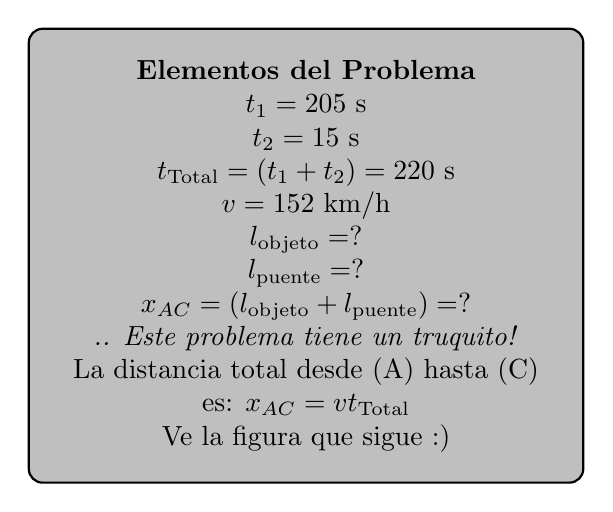
\begin{tikzpicture}
    \node[draw, line width=0.8pt, rounded corners=5pt, fill=lightgray, inner sep=10pt] (box) {
        \begin{tabular}{c}
            \textbf{Elementos del Problema} \\
            $t_{1}=205$ s \\
            $t_{2}=15$ s \\
            $t_{\text{Total}}=(t_{1}+t_{2})=220$ s \\
            $v=152$ km/h \\
            $l_{\text{objeto}}=?$ \\
            $l_{\text{puente}}=?$ \\
            $x_{AC}=(l_{\text{objeto}}+l_{\text{puente}})=?$ \\
            \textit{.. Este problema tiene un truquito!} \\
            La distancia total desde (A) hasta (C) \\
            es: $x_{AC}=vt_{\text{Total}}$ \\
            Ve la figura que sigue :)
        \end{tabular}
    };
\end{tikzpicture}
\end{center}

% Adding the small drawing with text below the box
\vspace{0.5cm}
\begin{center}
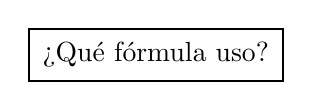
\begin{tikzpicture}
    \node[draw, line width=0.8pt, inner sep=5pt] at (0,0) {¿Qué fórmula uso?};
\end{tikzpicture}
\end{center}

% ============================================================== 
%----------------------------------------------------------------
%----------------------------------------------------------------
\end{frame}

\end{document}
